\clearpage
\section{Tópicos de pesquisa a serem investigados}
\label{ch:proposal}

This section presents some main ideas for the continuity of this doctoral
research project. \autoref{sec:topics} brings the research topics to be
addressed while \autoref{sec:timetable} shows the work plan and timetable.

%=============================================================================%
\subsection{Topicos de pesquisa}
\label{sec:topics}

%Devido ao compartilhamento de ambientes de rede, a natureza do \textit{best-effort} da infraestrutura da Internet, e o comportamento egoísta totalmente isolado dos jogadores da HAS discutidos na seção 3. É difícil para streams de vídeo satisfazer os três objetivos descritos abaixo. Desde de que existam multiplos clientes concorrentemente competindo entre eles um limitado comprimento de onda, as soluções existentes para clientes dirigido a HAS não trabalham vem e sofrem muitos problemas com perda de pacotes, flutação de comprimento de onda, oscilações na qualidado e troca de taxas de bits~(Instabiliddade do vídeo mostrada ba Figura~\TODO{Falta gerar gráfico}), QoE indesejavel e compartilhamento de recursos da rede, recursos da rede inutilizados ou sobrescritos do qual 'will adversely affect the viewer's QoE'.% Alem disso, estes problemas tem sido confirmados em experimentos recentas. 

The research topics to be addressed are divided into three topics, which are
detailed in Sections~\ref{subsec:distributed} through \ref{subsec:handover}.
Each topic encompasses the motivation, goals, and objectives.

%-----------------------------------------------------------------------------%
\subsubsection{Gerenciamento de mobilidade distribuída}
\label{subsec:handover}

O gerenciamento de mobilidade refere-se a um conjunto de mecanismos para manter a continuidade das sessões em andamento, enquanto um usuário móvel altera seu ponto de ancoragem da mobilidade na rede.
Na arquitetura DASH, as soluções de gerenciamento de mobilidade dependem de entidades âncoras de mobilidade centralizadas, responsáveis pelo plano de controle relacionado à mobilidade e pelos dados do usuário encaminhamento. 
%De acordo com~\citet{Valtulina2014}, essa abordagem centralizada torna o gerenciamento de mobilidade propenso a várias limitações de desempenho, como roteamento abaixo do ideal, baixa escalabilidade, potencial ponto único de falha e falta de granularidade para o serviço de gerenciamento de mobilidade.

%item Inicialmente, os parâmetros avaliados considerados incluem o perfil do usuário, a carga da célula local, a qualidade do link, a complexidade do movimento dos vídeos e também detalhes inteligentes da cidade, como a localização e a rota rastreada no caso de usuários com mobilidade. Alguns dos nós podem ser estacionários, mas outros podem variar de padrões de baixa a alta mobilidade, que podem ser levados em consideração para melhorar a qualidade da entrega de vídeo.

\emph{Os objetivos deste tópico de pesquisa são:}
\begin{itemize}

\item Realizar um estudo detalhado em soluções disponíveis para balanceamento de carga em redes móveis, que podem ser usadas para acionar procedimentos de transferência na arquitetura multinivel;

\item Examinar quais mecanismos existentes que devemos utilizar/desenvolver para lidar com a mobilidade do usuário.
Como dividir o conteúdo e recursos computacionais;

\item Analise as soluções existentes para transferência vertical em redes multiniveis, cuidando das transferências entre macro sobreposta e células pequenas;

\item Antes de alocar o serviço de streaming de video em DASH, quais serviços é necessário
acrescentar para o provisionamento do conteúdo

\end{itemize}


%-----------------------------------------------------------------------------%
\subsubsection{Mecanismos Cooperativos para Streaming de Video}
\label{subsec:video-streaming}


Em um ambiente de rede compartilhado, em que muitas entidades do sistema, incluindo players DASH, competem pela largura de banda disponível, várias flutuações repentinas na banda da rede podem ocorrer ao longo do tempo.

A seção~\ref{subsec:evaluation} mostra a influencia na variação entre diferentes processos de decisão para selecionar o bitrate do proximo segmento entre diferentes mecasnismos ABR. Em~\cite{bentaleb:2018:MSys} também mostram armadilhas devido ao comportamento totalmente isolado dos clentes HAS~(ou seja, essas soluções estão funcionando independentemente, sem coordenação). Em particular, a presença de vários clientes HAS simultâneos que competem pelos recursos de rede compartilhados podem cousar problemas de escalabilidade do HAS, incluindo (i) instabilidade de video devido à troca de taxa de bits frequente, na qual cinco players dash.js competem por um link de gargalo de 25 Mbps em um ambiente de rede compartilhado e oscilações de qualidade, como mostra a Figura 1.5; (ii) injustiça de QoE; e (iii) subutilização ou subscrição excessiva de recursos de rede. Esses problemas são agravados ainda mais quando o número de jogadores aumenta e no caso de ambientes heterogêneos. Esses problemas continuam sendo uma preocupação séria para os operadores de rede e provedores de conteúdo.

Neste contexto, é desejado ter um mecanismos computacionais que identifiquem automaticamente o processo de decisão do HAS de cada video antes de escalonar os videos.


O objetivo neeste topico de pesquisa é implementar mecanismos cooperativos capazes de identificar eficientemente o prcesso de decisão de cada cliente. Alem disso, esses mecanismos podem facilitar a coopereção de download e upload de um mesmo conteudo entre os usuários de uma mesma rede. Para isso, será implementado utilizando Teoria dos Jogos~(GT) composto por três estágios principais: entrada, processamento e saída. Os requisitos de QoE do video constituirão as entradas do sistema. Essas entradas serão mapeadas para as funções apropriadas de associação e valores de verdade.


%-----------------------------------------------------------------------------%
\subsubsection{Scalable controller architecture}
\label{subsec:sca}

Com a melhoria de largura de banda que foi feita nos links de acesso e nas redes de backbone, os usuários finais agora esperam que aplicativos de vídeo de alta qualidade funcionem em qualquer lugar e em uma variedade de dispositivos heterogêneos. Recentemente, como uma das novas arquiteturas de rede evolutiva, a Rede Centrada na Informação~(ICN)~[337] foi proposta para facilitar aplicativos como disseminação de conteúdo e serviços de streaming de alta qualidade (por exemplo, aplicativos de streaming de vídeo multicast baseados em HAS, etc.). No entanto, vários desafios, incluindo a cooperação com o cache na rede, o encaminhamento de múltiplos caminhos e o controle de qualidade ou congestionamento, ainda precisam ser enfrentados antes da implantação do serviço na Internet. De fato, a maioria dos trabalhos relacionados é baseado em várias suposições nas quais, por exemplo, aplicativos de destino são apenas aplicativos não em tempo real, a rede de destino deve ser uma pequena rede de gerenciamento ou uma rede com fio~(ou sem fio) e assim por diante. 

Paralelamente, a rede definida por software e a virtualização de funções de rede (SDN/NFV) são tecnologias notáveis para controlar não apenas os fluxos de comunicação, mas também as funções de serviço nas redes. Eles foram desenvolvidos recentemente por fornecedores internacionais e implantados no mercado. No entanto, como são basicamente projetados para funcionar com as redes IP ponto a ponto tradicionais, geralmente limitadas a um único sistema autônomo, elas requerem algumas extensões para permitir o streaming de vídeo de alta qualidade a um grande número de usuários heterogêneos na ampla Internet. 
Além disso, a tendência para a computação de borda e neblina deve ser integrada às abordagens de gerenciamento de tráfego de vídeo. Os recursos de borda dos ISPs ou usuários finais podem ser utilizados para hospedar o conteúdo de vídeo na proximidade dos usuários finais, reduzindo a latência e mitigando a carga nas redes principais e nos data centers. Isso será útil para o cenário de transmissão ao vivo que requer uma latência baixa. Além disso, a integração de serviços baseados em HAS em tais mecanismos de comunicação requer uma avaliação rigorosa em bancos de testes realistas antes da implantação. O principal objetivo é analisar e investigar a integração da entrega de vídeo baseada em HAS nas redes futuras, onde:


%
%\vspace{0.8cm}
%\begin{figure*}[htpb]
%	\centering
%	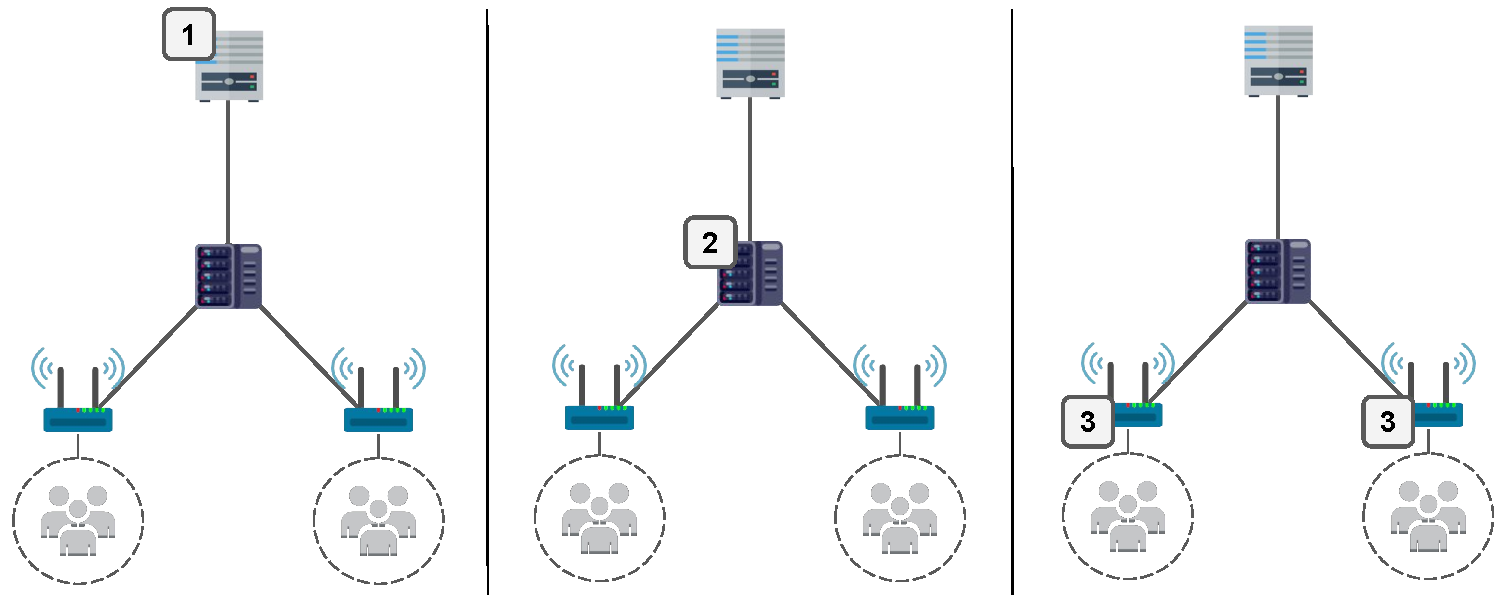
\includegraphics[width=0.75\textwidth]{img/exp-multi-lvl}
%% 	\vspace{-1cm}
%	\caption{DASH-based Adaptive Multimedia Delivery System for Cloud/Fog Nodes.}
%	\label{fig:scenario-arch}
%\end{figure*}


%-----------------------------------------------------------------------------%
\subsubsection{Scalable controller architecture}
\label{subsec:sca-contrl-arch}


Este projeto tem como objetivo projetar uma entrega de vídeo baseada em DASH confiável e de alta qualidade para ser usada em ambientes de cidades inteligentes~\cite{gamaUCC2019, KreuzbergerWorkshop2016}. O esquema proposto aproveitará várias tecnologias relacionadas à rede, como Cloud, Fog e Edge Computing, além de posicionamento e encadeamento inteligente de serviços.% A Figura~\ref{fig:scenario-arch} descreve, no lado esquerdo, uma arquitetura de rede de várias camadas, composta por um conjunto heterogêneo de dispositivos e aplicativos que utilizam recursos de computação distribuídos por meio de uma tecnologia de comunicação de acesso múltiplo, como 5G e WiFi. Este projeto propõe estender o streaming de vídeo DASH para suportar conectividade simultânea de caminhos múltiplos~\cite{poliakovPHD2018, Velasquez2018}.

%O lado direito da Figura~\ref{fig:scenario-arch} descreve parte dos parâmetros que devem ser avaliados para definir quais serviços de vídeo precisam ser implantados, juntamente com a camada mais adequada para implantar cada um deles. Observe que os parâmetros na camada mais inferior para feedback diferem dos de outras camadas. Inicialmente, os parâmetros avaliados considerados incluem o perfil do usuário, a carga da célula local, a qualidade do link, a complexidade do movimento dos vídeos e também detalhes inteligentes da cidade, como a localização e a rota rastreada no caso de usuários com mobilidade. Alguns dos nós podem ser estacionários, mas outros podem variar de padrões de baixa a alta mobilidade, que podem ser levados em consideração para melhorar a qualidade da entrega de vídeo.

\vspace{0.8cm}
\begin{figure*}[htpb]
	\centering
	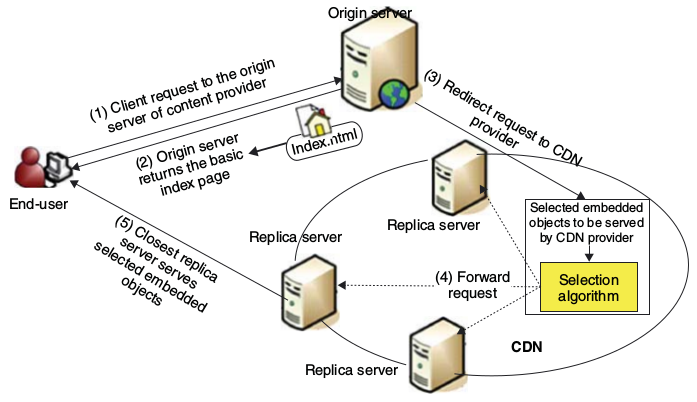
\includegraphics[width=0.7\textwidth]{img/fig-intro.png}
% 	\vspace{-1cm}
	\caption{DASH-based Adaptive Multimedia Delivery System for Cloud/Fog Nodes.}
	\label{fig:scenario-arch}
\end{figure*}

Dada a arquitetura do modelo de serviço e ambiente de nuvem/borda de várias camadas mencionada, este trabalho tem como objetivo abordar algumas das seguintes questões de pesquisa:~\textit{i)} Como determinar as melhores camadas para alocação de serviços de vídeo?~\textit{ii)} Como os pedaços de vídeo não solicitados devem ser distribuídos na hierarquia de borda/nuvem, considerando as informações de localização do usuário e estimativas sobre a localização futura do usuário em tempo real?~\textit{iii)} Como facilitar o streaming de vídeo através de várias fontes simultaneamente?~\textit{iv)} Como os algoritmos de adaptação à taxa de bits podem ser afetados pelo tamanho do pedaço de vídeo em uma arquitetura de várias camadas?

%\subsection{Multimedia Delivery System Schemes}
% Selection Algorithms

%\subsection{Game Theory Based Adaptative Bit Rate Scheme}

% This project aims to design a reliable and high-quality DASH-based video delivery to be used in Smart City Environments~\cite{gamaUCC2019, KreuzbergerWorkshop2016}. The proposed scheme will take advantage of several network-related technologies such as Cloud, Fog, and Edge Computing, as well as intelligent service placement and chaining. Figure~\ref{fig:scenario-arch} depicts, on its left-hand side, a multi-tier network architecture, which is composed of a heterogeneous set of devices and applications using distributed computing resources through a multi-access communication technology, such as 5G and WiFi. This project proposes to extend DASH video streaming to support simultaneous multipath connectivity~\cite{poliakovPHD2018, Velasquez2018}.

% The right-hand side of Figure~\ref{fig:scenario-arch} describes part of the parameters that should be assessed to define which video services are needed to be deployed along with the most suitable tier to deploy each of them. Note that the parameters in the bottommost tier for feedback differ from those of other tiers. Initially, the assessed parameters considered include the user's profile, the load of the local cell, the link quality, the motion complexity of the videos, and also smart city details such as the location and the traced route in case of users with mobility. Some of the nodes can be stationary, but others can range from low to high mobility patterns, which can be taken into account to improve quality of video delivery.

% \vspace{0.8cm}
% \begin{figure*}[htpb]
% 	\centering
% 	\includegraphics[width=1.0\textwidth]{images/scenario_incomplete}
% % 	\vspace{-1cm}
% 	\caption{DASH-based Adaptive Multimedia Delivery System in an Smart City Environment.}
% 	\label{fig:scenario-arch}
% \end{figure*}

% Neste trabalho, queremos construir um sistema CDN na fog com o uso de cache e sobreposição de rede para para streaming de video ao vivo, e otimizar sua topologia de forma adaptativa para minimizar a latência de reprodução média e melhorar a entrega do fluxo de forma oportuna. A latência de reprodução é a diferença entre o tempo de reprodução (ponto de reprodução) na origem de mídia e em um nó.

% \vspace{1cm}
% \noindent
% \textbf{Modelagem de propriedades de balanceamento de carga e desempenho de cache em sistemas de Névoa-Nuvem multicamadas.}

%-----------------------------------------------------------------------------%
%\subsection{Medidas objetivas}

%-----------------------------------------------------------------------------%
\subsubsection{Traffic offloading in \acsp{HetNet}}
\label{subsec:heterogeneous}

As the wireless link efficiency is approaching its fundamental limits, further
improvements in cellular system spectral efficiency are only possible by
increasing the node deployment density. As observed by \citet{Damnjanovic2011},
challenges associated with the deployment of traditional macro base stations
can be overcome by the utilization of base stations with lower transmit power.
A network that consists of a mix of macro cells and low-power nodes, where some
may be configured with restricted access and some may lack wired backhaul, is
referred to as a \acf{HetNet}. \autoref{fig:hetnet} exemplifies a \ac{HetNet}
with a macro cell, some metro and picocells used for relay, some network
operator deployed low-costs indoor and outdoor small cells, and user deployed
very low costs for indoor environment.

The future 5G architecture must provide a communication environment able to
overcome the infrastructure shortcomings of current networks. Networks will
become much denser with many more cells with decreasing size as well as direct
device-to-device communication. Small cells improve capacity and cellular
coverage with lower cost compared to macrocells, and they are expected to carry
the majority of traffic. \citet{Pierucci2015} says that while bringing the base
station closer to the user, it is possible to promote lower power use and more
energy efficient communications. In the opinion of \citet{Einsiedler2015}, the
vision is to provide functional convergence of network control to handle 5G,
4G, older access technologies, and Wi-Fi; enabling a flexible and efficient
support and deliver all types of applications.

\emph{The goal of this research topic is} to design an algorithm responsible
for offloading \ac{LTE} traffic over available Wi-Fi networks. Assuming that
many Wi-Fi hotspots are deployed by the mobile operators in public urban areas,
the algorithm focus is to trigger offloading decisions based on the current
traffic load in the backhaul and core networks.
\emph{The objectives for this research topic are:}
\begin{itemize}
  \item Compare current approaches for traffic offloading in mobile networks,
  identifying the benefits and drawbacks of each solution;

  \item Propose an improved offloading decision solution for \ac{EPC}, using
  Wi-Fi as enabler technology;

  \item Implement and evaluate the proposed solutions in the \ac{ns-3}
  simulator, performing tests on scenarios with different access networks.
\end{itemize}


\subsubsection{Modelagem de propriedades de balanceamento de carga e desempenho de cache
em sistemas de Névoa-Nuvem multicamadas}
\label{subsec:handover}

1. Interesses perspectivas do usuário, provedor de serviços e provedor de rede.
2. Qual a melhor forma de operar problemas de cache em névoa-nuvem? Onde? Quando?
Como?
3. Redimensionar recursos necessários para suportar demanda de Acordo com o tempo.
4. Utilizar máquinas virtuais (container, microservices) para atingir a latência minima para
acelerar a execução do escalonamento, mas irá implicar em desperdicios de recurso (e
dinheiro)? Caso sim, como minimizar este desperdicio?
105. Este trabalho aborda redes heterogêneas, com diferentes tipos de dispositivos. Como
cumprir os requisitos de QoS e QoE neste ambiente?
6. Quando um conteúdo é alocado na borda da rede quanto tempo o conteúdo deve perma-
necer na cache?

% Given the aforementioned multi-tier edge/cloud environment and service model architecture, this work aims to tackle some of the following research questions:~\textit{i)} How to determine the best tiers for video services placement?~\textit{ii)} How unsolicited video chunks should be distributed in the edge/cloud hierarchy considering user location information and estimates on future user location in real time? ~\textit{iii)} How to facilitate video streaming through multiple sources concurrently?~\textit{iv)} How bitrate adaptation algorithms can be impacted by video chunk size in a multi-tiered architecture?


%-----------------------------------------------------------------------------%
\subsubsection{Gerenciamento de mobilidade distribuída}
\label{subsec:handover}

O gerenciamento de mobilidade refere-se a um conjunto de mecanismos para manter a continuidade das sessões em andamento, enquanto um usuário móvel altera seu ponto de ancoragem da mobilidade na rede.
Na arquitetura DASH, as soluções de gerenciamento de mobilidade dependem de entidades âncoras de mobilidade centralizadas, responsáveis pelo plano de controle relacionado à mobilidade e pelos dados do usuário encaminhamento. 
%De acordo com~\citet{Valtulina2014}, essa abordagem centralizada torna o gerenciamento de mobilidade propenso a várias limitações de desempenho, como roteamento abaixo do ideal, baixa escalabilidade, potencial ponto único de falha e falta de granularidade para o serviço de gerenciamento de mobilidade.

%item Inicialmente, os parâmetros avaliados considerados incluem o perfil do usuário, a carga da célula local, a qualidade do link, a complexidade do movimento dos vídeos e também detalhes inteligentes da cidade, como a localização e a rota rastreada no caso de usuários com mobilidade. Alguns dos nós podem ser estacionários, mas outros podem variar de padrões de baixa a alta mobilidade, que podem ser levados em consideração para melhorar a qualidade da entrega de vídeo.

\emph{Os objetivos deste tópico de pesquisa são:}
\begin{itemize}

\item Realizar um estudo detalhado em soluções disponíveis para balanceamento de carga em redes móveis, que podem ser usadas para acionar procedimentos de transferência na arquitetura multinivel;

\item Examinar quais mecanismos existentes que devemos utilizar/desenvolver para lidar com a mobilidade do usuário.
Como dividir o conteúdo e recursos computacionais;

\item Analise as soluções existentes para transferência vertical em redes multiniveis, cuidando das transferências entre macro sobreposta e células pequenas;

\item Antes de alocar o serviço de streaming de video em DASH, quais serviços é necessário
acrescentar para o provisionamento do conteúdo

\end{itemize}

This project aims to design a reliable and high-quality DASH-based video delivery to be used in
Smart City Environments [1, 2]. The proposed scheme will take advantage of several network-
related technologies such as Cloud, Fog, and Edge Computing, as well as intelligent service
placement and chaining. Figure 1 depicts, on its left-hand side, a multi-tier network architecture,
which is composed of a heterogeneous set of devices and applications using distributed computing
resources through a multi-access communication technology, such as 5G and WiFi. This project
proposes to extend DASH video streaming to support simultaneous multipath connectivity [3, 4].


describes part of the parameters that should be assessed to define which video services are needed to be deployed along with the most suitable tier to deploy each of them. Note that the parameters in the bottommost tier for feedback differ from those of other tiers.
Initially, the assessed parameters considered include the user’s profile, the load of the local cell, the link quality, the motion complexity of the videos, and also smart city details such as the location and the traced route in case of users with mobility. Some of the nodes can be stationary, but others can range from low to high mobility patterns, which can be taken into account to improve quality of video delivery.

Mobility management refers to a set of mechanisms to keep ongoing sessions
continuity while a mobile user changes its mobility anchor point in the
network. In the \ac{LTE} architecture, mobility management solutions rely on
centralized mobility anchor entities (\ac{S-GW} and \ac{P-GW}), which are in
charge of both mobility-related control plane and user data forwarding.
According to \citet{Valtulina2014}, this centralized approach makes mobility
management prone to several performance limitations such as suboptimal
routing, low scalability, potential single point of failure and the lack of
granularity for the mobility management service.

\emph{The objectives for this research topic are:}
\begin{itemize}
  \item Detailed study of \ac{LTE} handover procedures to propose a suitable
  distribution among \ac{MME} and available OpenFlow controllers, considering
  the interoperability with \ac{3GPP} standards;

  \item Examine available solutions for load balancing in mobile networks,
  which can be used to trigger handover procedures in the distributed
  architecture;

  \item Analyze existing solutions for vertical handover in \acp{HetNet},
  taking care of handovers between overlapping macro and small cells;

  \item Assess approaches for rerouting tunnels in OpenFlow backhaul network,
  looking for an optimal anchor element;

  \item Implement and evaluate the proposed \ac{DMM} in the \ac{ns-3}
  simulator, performing handover tests with groups of \acp{UE} between
  \acp{eNB}.
\end{itemize}


%=============================================================================%
\subsection{Plano de trabalho}
\label{sec:timetable}


\autoref{tab:timetable} apresenta o cronograma para este projeto de pesquisa de doutorado. As atividades mencionadas no cronograma estão listadas abaixo e incluem o trabalho desenvolvido apresentado em \autoref{ch:develop} e os tópicos a serem investigados em \autoref{sec:topics}. As atividades já desenvolvidas são identificadas pelo símbolo~\,\m. Enquanto isso, o símbolo \,\x\ identifica o tempo esperado para a realização das atividades planejadas.

%\autoref{tab:timetable} presents the timetable for this doctoral research
%project. The activities referenced in the timetable are listed below and
%comprises both the developed work introduced in \autoref{ch:developed} and the
%topics to be investigated from \autoref{sec:topics}. The activities that are
%already developed are identified by the symbol~\,\m. Meanwhile, the symbol
%\,\x\, identifies the expected time for carrying out the planned activities.

\begin{enumerate}
%	\item cumprimento de créditos de disciplinas;
%	\item pesquisa bibliografica;
%	\item desenvolvimento do ambiente de simulação;
%	\item desenvolvimento do algoritmo base para RCSA;
%	\item testes de validação dos resultados parciais;
%	\item análise dos resultados parciais;
%	\item documentação e publicação dos resultados parciais;
  

  \item Estudo detalhado sobre a integração em redes multiniveis;
	\item formalização da metodologia de pesquisa;
  \item Avaliação de ferramentas de software disponíveis para análise de desempenho;
  \item Desenvolvimento do módulo libdash para \ac{ns-3};
  \item Escrita e defesa para exame de qualificação para doutorado;
  \item Proposta de arquitetura de controlador escalável;
  \item Offloading de tráfego em redes heterogêneas;
  \item Soluções de gerenciamento de mobilidade distribuída;
  	\item testes de validação dos resultados parciais;
	\item análise dos resultados parciais;
  \item Redação e defesa de tese.

%  \item Proposal of the \ac{SDN}-enabled \ac{LTE} network;
%  \item OpenFlow \ac{EPC} controller for traffic routing and bearer admission
%        control;
%  \item \ac{LTE} \ac{QoS} realization with OpenFlow protocol;
\end{enumerate}

\begin{table}[htb]
  \renewcommand{\arraystretch}{1.4}
  \caption{The timetable for this doctoral research project.}
  \label{tab:timetable}
  \tiny
  \centering
  \begin{tabular}{c|c|cccc|cccc|cccccc|c}
    \toprule
    & {\bf 2017}
    & \multicolumn{4}{c|}{{\bf 2018}}
    & \multicolumn{4}{c|}{{\bf 2019}}
    & \multicolumn{6}{c|}{{\bf 2020}}
    & {\bf 2021} \\

    & {\it Oct} & {\it Jan} & {\it Apr} & {\it Jul} & {\it Oct} & {\it Jan} &
    {\it Apr} & {\it Jul} & {\it Oct} & {\it Jan} & {\it Mar} & {\it May} &
    {\it Jul} & {\it Sep} & {\it Nov} & {\it Jan} \\

    & {\it Dec} & {\it Mar} & {\it Jun} & {\it Sep} & {\it Dec} & {\it Mar} &
    {\it Jun} & {\it Sep} & {\it Dec} & {\it Feb} & {\it Apr} & {\it Jun} &
    {\it Aug} & {\it Oct} & {\it Dec} & {\it Feb} \\
    \hline % \midrule
    \arrayrulecolor{lightgray}

    %        |2013|       2014        |       2015        |            2016             |2017
    %        | 08 | 01   04   07   10 | 01   04   07   10 | 01   03   05   07   09   11 | 01
    %        | 12 | 03   06   09   12 | 03   06   09   12 | 02   04   06   08   10   12 | 02
    {\bf 01} & \m & \m &    &    &    &    &    &    &    &    &    &    &    &    &    &    \\ \hline
    {\bf 02} &    & \m &    &    &    &    &    &    &    &    &    &    &    &    &    &    \\ \hline
    {\bf 03} &    & \m & \m & \m & \m &    &    &    &    &    &    &    &    &    &    &    \\ \hline
    {\bf 04} &    &    &    & \m & \m & \m &    &    &    &    &    &    &    &    &    &    \\ \hline
    {\bf 05} &    &    &    &    &    & \m & \m & \m &    &    &    &    &    &    &    &    \\ \hline
    {\bf 06} &    &    &    &    &    &    &    & \m & \m &    &    &    &    &    &    &    \\ \hline
    {\bf 07} &    &    &    &    &    &    &    &    & \x & \x &    &    &    &    &    &    \\ \hline
    {\bf 08} &    &    &    &    &    &    &    &    & \x & \x & \x &    &    &    &    &    \\ \hline
    {\bf 09} &    &    &    &    &    &    &    &    &    & \x & \x & \x & \x & \x &    &    \\ \hline
    {\bf 10} &    &    &    &    &    &    &    &    &    &    &    & \x & \x & \x & \x &    \\ \hline
    {\bf 11} &    &    &    &    &    &    &    &    &    &    &    &    &    & \x & \x & \x \\

    \arrayrulecolor{black}
    \bottomrule
  \end{tabular}
\end{table}



%=============================================================================%
%\section{Motivação}

%Este projeto propõe o uso da hierarquia de borda/nuvem para projetar um streaming de vídeo DASH cooperativo nas Smart Cities, implantando o serviço de cache para oferecer melhor qualidade de experiência~(QoE) para os usuários finais.
%At the same time, video streaming services represent the majority of the internet traffic, and according to Cisco forecasts\footnote{Cisco Visual Networking Index: Global Mobile Data Traffic Forecast Update. Link:~\url{http://shorturl.at/hjAZ1}. Accessed: July 29, 2019.}, in 2021 70\% of all internet traffic will be dominated by video streaming. This includes current video services as well as innovative services such as cloud gaming and future consoles (e.g. Google Stadia), whereas for mobile devices this estimate represents 78\% of all mobile data traffic. To accommodate video traffic, a good cloud-level architecture partially solves some issues related to the live stream and Video on Demand~(VoD) services. However, a centralized cloud service introduces some issues such as higher latency and core network congestion. Therefore, to improve video services, it is of paramount importance to properly distribute video streams according to their requirements: a cloud gaming infrastructure is an interactive service that needs reduced delays (a few milliseconds), while a non-interactive VoD delivery can tolerate higher delays without impairing quality of experience. A proper management and orchestration of video delivery over the Internet is core to the smooth co-existence of heterogeneous video services. This project proposes the use of edge/cloud hierarchy to design a cooperative DASH video streaming in Smart Cities, deploying cache service to offer improved Quality of Experience~(QoE) for end-users.

%*********** about IOT ******************


%***********Objectives of the proposal***********
%1. How to deliver high quality streaming using in-Network coding and caching?
%2. How to enable the multipath and multicast capabilities for HAS in future networks like ICN?
%3. What is the impact of these networks on HAS decisions?
%4. What is the benefits that edge computing can add in HAS over the future networks?
%5. What is the deployment cost?

%
%\section{Problem Statement}
%
%The most of the exiting HAS delivery solutions, and their ABR schemes have four major shortcomings which are summarized as follows:
%
%1. Multi-player problem.
%
%2. Bandwidth fluctuation problem.
%
%3. Quality fairness and heterogeneous system problem.
%
%4. Trade-off between QoE metrics and ABR objectives problem.
